%%%%%%%%%%%%%%%%%%%%%%%%%%%%%%%%%%%%%%%%%%%%%%%%%%%%%%%%%%%%%%%
%% BRIEF VERSION OF OXFORD THESIS TEMPLATE FOR CHAPTER PREVIEWS

%%%%% CHOOSE PAGE LAYOUT
% format for PDF output (ie equal margins, no extra blank pages):
\documentclass[a4paper,nobind]{templates/ociamthesis}

% UL 30 Nov 2018 pandoc puts lists in 'tightlist' command when no space between bullet points in Rmd file
\providecommand{\tightlist}{%
  \setlength{\itemsep}{0pt}\setlength{\parskip}{0pt}}
  
\usepackage{float}  
 
% UL 1 Dec 2018, fix to include code in shaded environments
\usepackage{color}
\usepackage{fancyvrb}
\newcommand{\VerbBar}{|}
\newcommand{\VERB}{\Verb[commandchars=\\\{\}]}
\DefineVerbatimEnvironment{Highlighting}{Verbatim}{commandchars=\\\{\}}
% Add ',fontsize=\small' for more characters per line
\usepackage{framed}
\definecolor{shadecolor}{RGB}{248,248,248}
\newenvironment{Shaded}{\begin{snugshade}}{\end{snugshade}}
\newcommand{\AlertTok}[1]{\textcolor[rgb]{0.94,0.16,0.16}{#1}}
\newcommand{\AnnotationTok}[1]{\textcolor[rgb]{0.56,0.35,0.01}{\textbf{\textit{#1}}}}
\newcommand{\AttributeTok}[1]{\textcolor[rgb]{0.77,0.63,0.00}{#1}}
\newcommand{\BaseNTok}[1]{\textcolor[rgb]{0.00,0.00,0.81}{#1}}
\newcommand{\BuiltInTok}[1]{#1}
\newcommand{\CharTok}[1]{\textcolor[rgb]{0.31,0.60,0.02}{#1}}
\newcommand{\CommentTok}[1]{\textcolor[rgb]{0.56,0.35,0.01}{\textit{#1}}}
\newcommand{\CommentVarTok}[1]{\textcolor[rgb]{0.56,0.35,0.01}{\textbf{\textit{#1}}}}
\newcommand{\ConstantTok}[1]{\textcolor[rgb]{0.00,0.00,0.00}{#1}}
\newcommand{\ControlFlowTok}[1]{\textcolor[rgb]{0.13,0.29,0.53}{\textbf{#1}}}
\newcommand{\DataTypeTok}[1]{\textcolor[rgb]{0.13,0.29,0.53}{#1}}
\newcommand{\DecValTok}[1]{\textcolor[rgb]{0.00,0.00,0.81}{#1}}
\newcommand{\DocumentationTok}[1]{\textcolor[rgb]{0.56,0.35,0.01}{\textbf{\textit{#1}}}}
\newcommand{\ErrorTok}[1]{\textcolor[rgb]{0.64,0.00,0.00}{\textbf{#1}}}
\newcommand{\ExtensionTok}[1]{#1}
\newcommand{\FloatTok}[1]{\textcolor[rgb]{0.00,0.00,0.81}{#1}}
\newcommand{\FunctionTok}[1]{\textcolor[rgb]{0.00,0.00,0.00}{#1}}
\newcommand{\ImportTok}[1]{#1}
\newcommand{\InformationTok}[1]{\textcolor[rgb]{0.56,0.35,0.01}{\textbf{\textit{#1}}}}
\newcommand{\KeywordTok}[1]{\textcolor[rgb]{0.13,0.29,0.53}{\textbf{#1}}}
\newcommand{\NormalTok}[1]{#1}
\newcommand{\OperatorTok}[1]{\textcolor[rgb]{0.81,0.36,0.00}{\textbf{#1}}}
\newcommand{\OtherTok}[1]{\textcolor[rgb]{0.56,0.35,0.01}{#1}}
\newcommand{\PreprocessorTok}[1]{\textcolor[rgb]{0.56,0.35,0.01}{\textit{#1}}}
\newcommand{\RegionMarkerTok}[1]{#1}
\newcommand{\SpecialCharTok}[1]{\textcolor[rgb]{0.00,0.00,0.00}{#1}}
\newcommand{\SpecialStringTok}[1]{\textcolor[rgb]{0.31,0.60,0.02}{#1}}
\newcommand{\StringTok}[1]{\textcolor[rgb]{0.31,0.60,0.02}{#1}}
\newcommand{\VariableTok}[1]{\textcolor[rgb]{0.00,0.00,0.00}{#1}}
\newcommand{\VerbatimStringTok}[1]{\textcolor[rgb]{0.31,0.60,0.02}{#1}}
\newcommand{\WarningTok}[1]{\textcolor[rgb]{0.56,0.35,0.01}{\textbf{\textit{#1}}}}

%UL 2 Dec 2018 add a bit of white space before and after code blocks
\renewenvironment{Shaded}
{
  \vspace{4pt}%
  \begin{snugshade}%
}{%
  \end{snugshade}%
  \vspace{4pt}%
}
%UL 2 Dec 2018 reduce whitespace around verbatim environments
\usepackage{etoolbox}
\makeatletter
\preto{\@verbatim}{\topsep=0pt \partopsep=0pt }
\makeatother

%UL 28 Mar 2019, enable strikethrough
\usepackage[normalem]{ulem}

%UL 3 Nov 2019, avoid mysterious error from not having hyperref included
\usepackage{hyperref}

%%%%% SELECT YOUR DRAFT OPTIONS
% Three options going on here; use in any combination.  But remember to turn the first two off before
% generating a PDF to send to the printer!

% This adds a "DRAFT" footer to every normal page.  (The first page of each chapter is not a "normal" page.)

% This highlights (in blue) corrections marked with (for words) \mccorrect{blah} or (for whole
% paragraphs) \begin{mccorrection} . . . \end{mccorrection}.  This can be useful for sending a PDF of
% your corrected thesis to your examiners for review.  Turn it off, and the blue disappears.

%%%%% BIBLIOGRAPHY SETUP
% Note that your bibliography will require some tweaking depending on your department, preferred format, etc.
% The options included below are just very basic "sciencey" and "humanitiesey" options to get started.
% If you've not used LaTeX before, I recommend reading a little about biblatex/biber and getting started with it.
% If you're already a LaTeX pro and are used to natbib or something, modify as necessary.
% Either way, you'll have to choose and configure an appropriate bibliography format...

% The science-type option: numerical in-text citation with references in order of appearance.
% \usepackage[style=numeric-comp, sorting=none, backend=biber, doi=false, isbn=false]{biblatex}
% \newcommand*{\bibtitle}{References}

% The humanities-type option: author-year in-text citation with an alphabetical works cited.
% \usepackage[style=authoryear, sorting=nyt, backend=biber, maxcitenames=2, useprefix, doi=false, isbn=false]{biblatex}
% \newcommand*{\bibtitle}{Works Cited}

%UL 3 Dec 2018: set this from YAML in index.Rmd
\usepackage[style=numeric-comp, sorting=none, backend=biber, doi=false, isbn=false]{biblatex}
\newcommand*{\bibtitle}{References}

% This makes the bibliography left-aligned (not 'justified') and slightly smaller font.
\renewcommand*{\bibfont}{\raggedright\small}

% Change this to the name of your .bib file (usually exported from a citation manager like Zotero or EndNote).
\addbibresource{}

\newlength{\cslhangindent}
\setlength{\cslhangindent}{1.5em}
\newenvironment{CSLReferences}%
  {}%
  {\par}
  
\newlength{\csllabelwidth}
\setlength{\csllabelwidth}{3em}

\usepackage{calc}
\newcommand{\CSLLeftMargin}[1]{\parbox[t]{\csllabelwidth}{#1}}
\newcommand{\CSLRightInline}[1]{\parbox[t]{\linewidth - \csllabelwidth}{#1}\break}
\newcommand{\CSLIndent}[1]{\hspace{\cslhangindent}#1}

%%%%% YOUR OWN PERSONAL MACROS
% This is a good place to dump your own LaTeX macros as they come up.

% To make text superscripts shortcuts
	\renewcommand{\th}{\textsuperscript{th}} % ex: I won 4\th place
	\newcommand{\nd}{\textsuperscript{nd}}
	\renewcommand{\st}{\textsuperscript{st}}
	\newcommand{\rd}{\textsuperscript{rd}}

%%%%% THE ACTUAL DOCUMENT STARTS HERE
\begin{document}

%%%%% CHOOSE YOUR LINE SPACING HERE
% This is the official option.  Use it for your submission copy and library copy:
\setlength{\textbaselineskip}{22pt plus2pt}
% This is closer spacing (about 1.5-spaced) that you might prefer for your personal copies:
%\setlength{\textbaselineskip}{18pt plus2pt minus1pt}

% UL: You can set the general paragraph spacing here - I've set it to 2pt (was 0) so
% it's less claustrophobic
\setlength{\parskip}{2pt plus 1pt}

% Leave this line alone; it gets things started for the real document.
\setlength{\baselineskip}{\textbaselineskip}

% all your chapters and appendices will appear here
\begin{savequote}
Science knows it doesn't know everything; otherwise, it'd stop.
\end{savequote}



\hypertarget{background-heading}{%
\chapter{Background \& Objectives}\label{background-heading}}

\minitoc 

\hypertarget{lay-summary}{%
\section{Lay summary}\label{lay-summary}}

Around \textbf{{[}NUMBER{]}} people in the UK live with dementia, and by 2040, nearly twice as many will have the condition. No cure for dementia exists, so researchers are trying to find ways to prevent the condition. This involves finding risk factors for dementia that we can change. Risk factors increase a person's risk of developing a disease. Avoiding a risk factor does not guarantee that a person will not develop dementia, but makes it less likely. A key risk factor for dementia may be the levels of lipids (fatty substances such as cholesterol) in a person's blood. However, researchers remain unsure, as studies disagree on whether a role for lipids in dementia exists.

Additionally, because of problems in the design of previous studies, a cause and effect link between lipids and dementia could not be confirmed.

The research contained in this thesis will sum up what we know about the relationship between lipids and dementia.

I will use all available evidence, including that preprinted by authors (i.e.~not formally reviewed by others in their field to assess the accuracry of their claims) to assess whether lipid levels cause dementia.

Finally, I will attempt to find the groups of patients that might benefit most from treatment to change their lipid levels.

\hypertarget{introduction}{%
\section{Introduction}\label{introduction}}

This Chapter will provide an overview of the thesis, introducing the core concepts used throughout and providing some background context on each. It will briefly discuss the natural history of dementia, it's public health importance and the

In this context it will highlight the importance of identifying easily modified risk factors, and introduce blood lipids, and blood lipid-modifying treatements such as statins, as the primary exposures e

It will also introduce the primary exposures used in this thesis, covering the biological role, measurement and. It will cover the mechanism of common lipid regulating agents.

Finally, it will outline the theoretical framework used in this thesis.

\hypertarget{dementia}{%
\section{Dementia}\label{dementia}}

Dementia is a progressive neurocognitive disorder, characterised by impaired memory, reduced executive function and

A

The most common types of which are Alzheimer's disease (AD) and vascular dementia (VaD) {[}1{]}.

Several cardiovascular elements have been identified as potential risk factors for dementia, and of these, lipid levels represent a promising target for preventative intervention due to the availability of lipid-modifying treatments. In this context, determining whether variations in lipid levels are causative for dementia may prove critical in reducing the future burden of the condition.

Dementia is major neurocognitive disorder, with symptoms including impairment of executive cognitive functions such as speech, judgement and memory. The most common causes of dementia are Alzheimer's disease and vascular dementia, accounting for \textasciitilde60-80\% and \textasciitilde10\% of cases respectively. The remaining 10-30\% of cases are caused other dementia subtypes (e.g.~Lewy Body dementia) or by progression of other neurological diseases (e.g.~Parkinson's disease).

Two important considerations on the

Dementia is difficult to diagnose, primarily due to the absence of a gold standard test for the condition. Information from multiple diagnostic tools are utilised, from medical history examination, through assessment of patients mental ability (e.g.~the Mini-Mental State Examination), to clinical tests (e.g.~Magnetic Resonance Imaging (MRI) scans).

\hypertarget{public-health-importance}{%
\subsection{Public Health importance}\label{public-health-importance}}

Dementia is quickly becoming a critically important public health issue. Despite the age-specific incidence and prevalence of dementia remaining relatively constant over time,{[}@prince2016{]} an ageing population looks set to create a dementia epidemic, particularly in Westernised countries. While approximately have received a dementia diagnosis, the true number of people currently living with dementia in the UK is thought to be closer to 850,000, with this figure expected to double by 2040.{[}@baker2019{]} Globally, the prevalence of dementia is expected to reach 75 million by 2030.{[}@prince2016{]} Despite the increasing number of dementia cases and decades of research, there remains much unknown about the pathogenesis and progression of the disease.

\hypertarget{chronic-underfunding}{%
\subsection{Chronic underfunding}\label{chronic-underfunding}}

Despite it's

Statistic comparison

Given all of this, the systematic assessment of easily modifiable targets (such as blood lipid levels) for their utility in the prevention of dementia should be considered.

\hypertarget{natural-history}{%
\subsection{Natural history}\label{natural-history}}

Much remains unknown about dementia pathogenesis, despite research implicating amyloid plaques and neurofibrillary tangles as potential mechanisms of disease {[}2{]}. Progression from onset is an average

\hypertarget{alzheimers-disease}{%
\subsection{Alzheimer's disease}\label{alzheimers-disease}}

Named after Aloi

\hypertarget{vascular-dementia}{%
\subsection{Vascular dementia}\label{vascular-dementia}}

Second largest underlying pathology of dementia

Diagnosed using the NINCDS-AIREN criteria.{[}@roman1993vascular{]}

\hypertarget{diagnostis-criteria}{%
\subsection{Diagnostis criteria}\label{diagnostis-criteria}}

There exist several diagnostic criteria for dementia and related disease, many of which have existed for quite some time and have more recently been updated to reflect current understanding in deme.

In all cases, dementia is diagnosed on the basis of behavioural.

it is a inherently subjective diagnosis made by an experience clinican. This means the potential for misclassification both of dementia vs no-dementia and between the different underlying conditions is extremely likely.

\begin{table}[!h]

\caption{\label{tab:diagnosticCriteria-table}Diagnostic criteria used to diagnose different types of dementia}
\centering
\begin{tabular}[t]{lll}
\toprule
Disease & Criteria & Summary\\
\midrule
AD & NINCDS-ADRDA & Lorem ipsum\\
VaD & NINCDS-AIREN & Lorem ipsum 2\\
\bottomrule
\end{tabular}
\end{table}

Several sets of criteria are commonly used to diagnose dementia, and the underlying diseases for research purposes. Two of the most commonly used include the criteria of the Diagnostic and Statistical Manual of Mental Disorders, fourth edition (DSM-IV-TR)1 and the National Institute of Neurological Disorders and Stroke--Alzheimer Disease and Related Disorders (NINCDS-ADRDA).{[}@dubois2007{]}

{[}\textbf{Need first NINCDS-ADRDA citation and DSM-IV citations}{]}

While these criteria define the, they are informed using practical scales to measure patients cognitive health.

One of the best known of thes scales is the

A further sclae is the MoCA

Also touch on aspects of each, such as the clock-drawing and whether or not they need to validated with input from another person.

The distinction between memory scales and dementia diagnosis scales should be noted, and the common confluence of the two addressed.

For example MMSE scores is a tool for assessing cognitive impairment, but does not by itself indicate the absence or presence of dementia. A low score on the MMSE should feed into the diagnostic process, potentiall as a screenign tool to help identify which patients require further assessment by a trained clinican. Studies that use it alone are likely to be biased.

Differentiating between the underlying causes of a dementia diagnosis is challenging but necessary, as whether the patient has Alzheimer's disease or vascular dementia will affect expect progression and potential treatment options available.

\hypertarget{differing-risk-by-sex}{%
\subsection{Differing risk by sex}\label{differing-risk-by-sex}}

Transparency guidelines that suggest sex should eb treated as biological variable and so results should be presented stratified t

Rate of dementia/AD differs in men and women

Previous studies have hinted that the relationship is dependent on individual-level characteristics such as age and sex {[}16,28{]}.

\hypertarget{challenges-in-the-study-of-dementia-using-traditional-study-designs}{%
\section{Challenges in the study of dementia using traditional study designs}\label{challenges-in-the-study-of-dementia-using-traditional-study-designs}}

Speak to the

Historically, studies on dementia have faced a range of challenges. As a range of determinants (genetic, environmental and lifestyle) are thought to jointly influence the risk, progression and outcomes of dementia, any individual association is likely to have only a small effect. Therefore, the statistical power need to detect these associations will often require sample sizes that are unfeasible using primary data collection. This fact is further complicated by the long latency of dementia, which necessitates a costly long-term approach to patient follow-up. Furthermore, dementia studies often have limited generalisability to the target population, as certain subgroups (e.g.~the very old) are frequently under-represented in study cohorts due to difficulties associated with their recruitment.9 Finally, studies employing a case-control design are further limited by the high potential for differential recall bias between those who have and have not developed dementia.10

Fortunately, these limitations may potentially be addressed through the use of routinely collected health data, and the electronic health record databases in which they are stored.

\emph{Cognitive impairment not dementia} (CIND) is another term used to described those with cognitive impairment but who fall below the diagnostic criteria for dementia.

A further clinical subtype that is of particular import the

And MCI

hr

\hypertarget{economic-impact}{%
\subsection{Economic impact}\label{economic-impact}}

The economic impact of dementia is enormous, but in terms of the direct care required

Patients with dementia stay in hospital for longer,{[}@mollers2019{]}

Patients are more prone to falls and other con

Costs can be categorised as direct and indirect, in terms of direct costs of hospitalisations an, but alos in terms of caring responsibilities for those re

\hypertarget{treatments}{%
\subsection{Treatments}\label{treatments}}

At present, there are no known curative treatments for dementia, though several

Development treatments for dementia is regularly deemed to be one of the hardest markets in the pharmaceultical world, given the overall lack of success of multiple promining therapeutics.

\hypertarget{risk-factors-and-preventative-measures}{%
\subsection{Risk factors and Preventative measures}\label{risk-factors-and-preventative-measures}}

Given the lack of available treatments, a strong focus has landed on preventative measures for dementia.

Several elements are considered to be risk factors for subsequent dementia risk.

These

\hypertarget{serum-lipids}{%
\section{Serum lipids}\label{serum-lipids}}

Cholestorol

Basic cholesterol structure is a steroid nucleus

Cholesterol is a fat soluble molecule, meaning that

\hypertarget{range-of-lipids}{%
\subsection{Range of lipids}\label{range-of-lipids}}

The blood profile has a range of lipid fractions to it. However, for the sake of this thesis, we will only consider the three most important fractions, namely total cholesterol, low density lipoprotein cholesterol (LDLc), high density lipoprotein cholesterol (HDLc) and trigylcerides (TG).

Range of other higher and lower density

\hypertarget{total-cholesterol}{%
\subsection{Total cholesterol}\label{total-cholesterol}}

Total serum cholesterol is a summary measures, derived from the measure c

Total cholesterol can be measured directly. Minimal clinical difference in measurements between fasting and non-fasting states.

\hypertarget{triglycerides}{%
\subsection{Triglycerides}\label{triglycerides}}

These are the smallest/simplest type of lipids and so should go first, then build up to more complex phospholipids like LDL-c, HDL-c.

Triglycerides are a simple molecule

\hypertarget{hdl-c}{%
\subsection{HDL-c}\label{hdl-c}}

Cholesterol ratio

\hypertarget{ldl-c}{%
\subsection{LDL-c}\label{ldl-c}}

LDL-c levels are not directly measured but instead are estimated from using the Friedewald formula,{[}@friedewald1972{]} where the:

\[LDLc \approx TC - HDLc - kTG\] where \(k\) is 0.20 if measurements are in mg/dl and 0.45 if in mmol/l.

Limitations to the method include a requirement to fast for 12-14hrs prior to measures, an inability to estimate LDLc if TG levels are high

\hypertarget{statins}{%
\subsection{Statins}\label{statins}}

Statins are by far away the most common method of modufthe primary

Statins inhibit the conversion of 3-Hydroxy-3-Methylglutaryl-Coenzyme-A (HMG-CoA) into mevalonic acid, by compeitivlely binding with HMG-CoA Reductase (HMG-CoA-R). This conversion is the key rate limiting step in the biochemical pathway that produces cholesterol (see Figure \ref()), allowing statins to reduce prevention of cholesterol





\begin{figure}
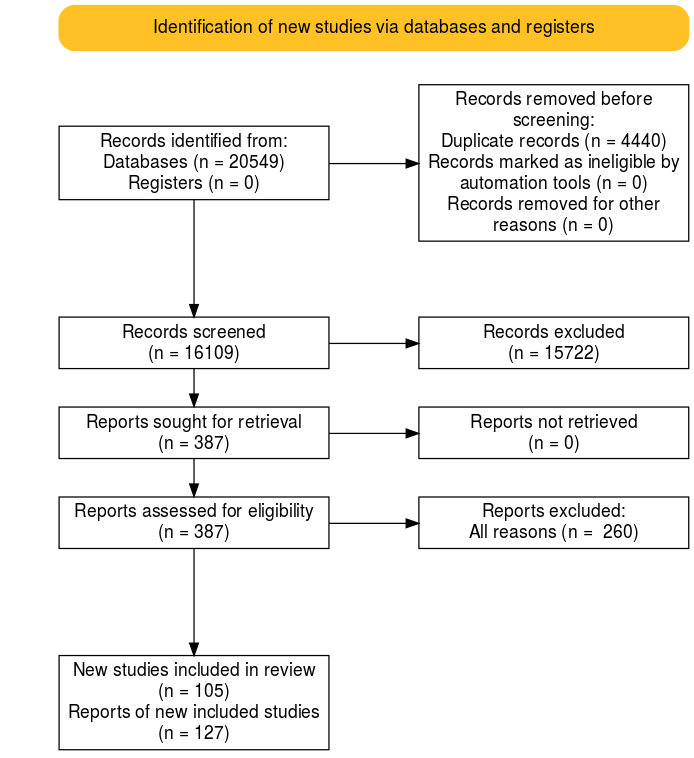
\includegraphics[width=1\linewidth]{figures/sys-rev/prisma_flow} \caption[Statin mechanism of action]{\textbf{Statin mechanism of action:}}\label{fig:statin-mechanisam}
\end{figure}

\hypertarget{lipophilic}{%
\subsubsection{Lipophilic}\label{lipophilic}}

Lipophic

Lipophilic statins are particularly important in the context of dementia, as they are able to cross the blood-brain barrier.

\hypertarget{hydrophilic}{%
\subsubsection{Hydrophilic}\label{hydrophilic}}

\hypertarget{other-lipid-regulating-agents-lra}{%
\subsection{Other lipid regulating agents (LRA)}\label{other-lipid-regulating-agents-lra}}

There are a range of other interventions that can be used to modify a persons lipid profile, though each act is slightly different want

For example, ezetimibe

\hypertarget{evidence-synthesis}{%
\section{Evidence synthesis}\label{evidence-synthesis}}

From a brief scoping literature search, Systematic reviews of the literature exist, with two main caveats: \textbf{{[}CITATION NEEDED - REFER to MSc project{]}}

Firstly, the majority of reviews

\hypertarget{thesis-focus-integrating-diverse-sources-of-evidence}{%
\section{Thesis focus: Integrating diverse sources of evidence}\label{thesis-focus-integrating-diverse-sources-of-evidence}}

The main theoretical framework used in this thesis is evidence synthesis - the discovery and critical integration of all available evidence on a research question in order to either: a) provide a more definitive answer to that question or; b) highlight gaps in the existing evidence base, so that future research address questions that have yet to be answered, or explores the same question in a way that increases our confidence in the result.

All elements of this thesis are based around this framework.

And the aim to integrate diverse sources of evidence. By diverse here,

Of particular interest is the synthesis of evidence from a range of diverse soources,

The main theoretical framework used in this thesis is evidence synthesis - the identification, critical assessment, and integration of all available evidence on a research question in order to either: a) provide a more definitive answer to that question; or b) highlight gaps in the existing evidence base.

While this thesis does include a research tool Chapter \ref{sys-rev-tools} and a primary evidence generation element (Chapter 5 - observational analysis of CPRD data), this was performed with the intention of providing a further source of evidence for the evidence synthesis/triangulation aspect of the thesis.

More specifically this includes the accurate searching of sources of grey literature (as enabled by the too presented in Chapter \ref{sys-rev-tools-heading}) and risk of bias assessment.

\hypertarget{study-designs-and-sources-of-bias}{%
\subsection{Study designs and sources of bias}\label{study-designs-and-sources-of-bias}}

Meta-analyses of randomised controlled trials are commonly seen as the gold standard in the

Indeed in the ``evidence pyramid'', meta-analysis of trials sit proudly on top. However, there included several potential limitations to this trial-only approach.

RCTs may be unfeasible if the outcome of interest is one with a long prodomal period, such as dementia, as they would require exteremely long and costly follow-up.{[}@ritchie2015{]}

Additionally randomised trials require clinical equipoise - something that is unlikely in the case of statins, as while equipose may exist, it would be unethical to randomised patients to statins or not given their proven protective effect against coronary disease.

It is no surprise then that the two know existing trials of statins for the prevention of dementia are in fact trials of statins for the prevention of coronary related outcomes.{[}@mcguinness2016a{]} The Prospective Study of Pravastatin in the Elderly (PROSPER) examined the protective effect of pravastating on coronary outcomes,

However, while being widely cited and indeed included in a Cochrane review on this topic (ironically, the lead author on this Cochrane review is ), these studies have major limitations that their utility to provide evidence on the effect of statin treatment on in assessing the impact of lipid-lowering treatment on dementia risk.

Firstly, there was no clinical cognitive evaluation of patients to . In fact, the PROSPER trial reported not on dementia outcomes, but on the change in cognitive scores over a mean of 3.2 years. As highlighted in Section @() , change in scores alone is insufficient to diagnose a dementia outcome.

The second trial, the Medical Research Council/British Health Foundation Protection Study

Additionally, there two trials, whiel putatively examining all cause dementia subject to the limitation described above, do not make any effort to assign an underlying pathogy to each case.

As discussed in Section

\textbf{Maybe take a stand here - and in the systematic review, and say that you are not going to }

There exist only two large scale randomized controlled trials of the effect of statins on dementia risk {[}CITE{]} - in fact these studies are the only two trials included in a 2016 review of statins for the prevention of dementia produced by the Cochrane {[}@mcguinness2016b{]}. Both showed no effect of

Queries around how the data were collected, along

A role for lipids in the aetiology of dementia is supported by both genetic linkage studies and functional cell biology studies. The generation of the amyloid plaques found in the brains of Alzheimer's patients is cholesterol dependent {[}CITE{]}, while the most established genetic risk factor for late-onset dementia, apolipoprotein E (ApoE), is involved in cerebral cholesterol transport. Several other genes involved in cholesterol transport have also been found to be robustly associated with increased AD susceptibility {[}CITE{]}.

Despite these encouraging results, evidence from epidemiological studies to date has been anecdotally been contradictory.

Several observational studies have examined the relationships between concentrations of serum lipids (total cholesterol (TC), low density lipoprotein cholesterol (LDL-c), high density lipoprotein cholesterol (HDL-c) and triglycerides) and both Alzheimer's disease and vascular dementia and reported widely different results. A high serum cholesterol concentration has been found to be associated with an increase in susceptibility to AD {[}8-13{]}, though other studies have shown no association {[}14-17{]}, or a reduced susceptibility {[}18,19{]}. With regards VaD, decreased levels of HDL-c appear to be associated with increased risk {[}18,20,21{]}, while for LDL-c, studies have reported both positive and negative association {[}18,22{]}.

Observational studies do not represent the only source of evidence examining the link between lipid levels and dementia. A recent Cochrane review identified two large randomised controlled trials (RCTs) of statins for the prevention of dementia, indicating that assignment to late-life lipid modifying treatment, as a proxy for lower lipid levels, does not reduce dementia risk {[}23{]}. However, both RCTs were limited, primarily by the relatively short follow-up period examined, while one failed to report the criteria used to diagnose dementia {[}24,25{]}. Finally, as they included only patients at high vascular risk, their generalisability to other settings is limited {[}23{]}.

Comment here on the use of MR studies as a different approach - one that is growing and commonly preprinted.

The use of newer methodological approaches, such as Mendelian randomisation (MR), has also produced contradictory results. In brief, MR uses genetic variants that are both strongly associated with the exposure of interest and are independent from potential confounders to strengthen causal inference {[}26{]}. A recent MR study indicated that low levels of LDL-c may cause a reduction in AD risk {[}27{]}. However, this study was criticised as it did not exclude the region surrounding the ApoE gene, meaning the risk reduction observed could be driven by variants in this region.

n short, each individual epidemiological approach taken to examine this research question is subject to distinct biases and short-comings that limit our ability to infer a causal relationship between blood lipids and subsequent dementia risk. However, as each approach will be subject to distinct biases, these differences in design can be advantageous. If all approaches point, or triangulate, towards the same answer, this strengthens the evidence of a causal link between lipid levels and dementia risk {[}26{]}. In this context, systematically identifying, assessing and integrating all available evidence in a triangulation framework, regardless of study design or approach taken, may help to increase our confidence that a causal relationship truly exists.

This thesis aims to find all exisiting evidence on the relationship between lipids/statins and dementia, critically assess it using a domain based tool

And then triangulate the different sources of evidence along with the primary analyses performed in this thesis.

\hypertarget{different-sources-of-bias}{%
\subsection{Different sources of bias}\label{different-sources-of-bias}}

While we can expect different study designs, this thesis also considers diverse sources of evidence in terms of the methodological approaches taken within a

The term ``observational study'', unlike RCT, belies wide range of analytical approaches,{[}@thiese2014{]} each with it's own limitations which can

Of particular interest in the context of interventional research is immortal time bias.

\hypertarget{misclassification-bias}{%
\subsubsection{Misclassification bias}\label{misclassification-bias}}

Incredibly hard to diagnose dementia, and even if diagnosed dementia, how to distinguish between different subtypes.

When using code lists to define outcomes in large, population scale electronic health databases, evidence exists that there is wild misclassification between the

Misclassification can also affect studies of interventions through the intorudction of immortal time. Several high profile observational studies of the effect of statins on dementi.

\hypertarget{reverse-causation}{%
\subsubsection{Reverse causation}\label{reverse-causation}}

Reverse causation is where the assumed exposure in an analytical framework is actually the outcome. \textbf{{[}CITATION NEEDED{]}} In the case of lipids and dementia, a reverse casaul relationship would be observed by the early prodomal effects of dementia influencing a change

\hypertarget{ascertainment-bias}{%
\subsubsection{Ascertainment bias}\label{ascertainment-bias}}

When examining the effect of treatment on low-lying diseases, number of consultations has an impact.

In this context, evidence synthesis exercises must account for these threats to internal validity as part of the synthesis. However, many previous highly cited systematic reviews have now done so.

Given the range of biases that can be expected to effect studies into dementia, any evidence synthesis effort must take account of these and perform a robust risk of bias assessment to assess the internal validity.

A key issues here, particularly in the context of using statins as a proxy for blood lipid levels, is that there is a key distinction between internal validity and generalisability. One can be called the wrong answer to the right question, the other, the right answer to the wrong question.

Having identified a gap in the literature in the systematic review, both in terms of an absence of observational studies using the specific deisng and in an absence of data related to vascular dementia, in Chapter \ref{cprd-analysis-heading}, I aim to address this evidence gap and provide a further source of information for the triangulation in Chapter \ref{discussion-heading}

\hypertarget{preprints-versus-peer-reviewed-articles}{%
\subsection{Preprints versus peer-reviewed articles}\label{preprints-versus-peer-reviewed-articles}}

Preprints

Preprints have existed in several fields, such as the aRxiv in the field of physics and mathematics, but more recently. Preprint repositories exist for everything from ecology (EcoEvoRxiv) to meta-research (metaArXiv)

Preprints can

Comment on good concordance between preprinted and published versions

There is much ongoing debate in, particulary in light of the explosion of prep

The outlook on this topic has shifted noticeab

One of the major criticisms of preprints is that they have not yet undergone formal peer review. Some researchers recommend treating

However, t

Additionally, in the context of systematic review. This however, substantially increases the need for thourough and detailed risk-of-bias assessment as part of a systematic review. In theory this should be donw anyways, but several of the existing highly cited reviews of observationsal studies of the relationship between tstatins and dementia did not perform a risk-of-bias assessment, or used

Checklists for risk of bias domains

However, the a noticeable s

One of the major current limitations for inclusion of data from preprint repositories in systematic reviews is the absence of a replicable and transparent search tool for performing systematic searches. The tool presented in Chapter \ref{sys-rev-tools} aims to address this.

\hypertarget{summary-level-results-vs-existing-un-analysed-datasets}{%
\subsection{Summary level results vs existing un-analysed datasets}\label{summary-level-results-vs-existing-un-analysed-datasets}}

Analysis of summary level data, that is the data extracted from publications describing primary studies, can only take investigations so far.

We are limited to the question that the original investigators wanted to ask, and the summar statistics they choose to present (see Section , which contributed to a discursive piece on present summary statistics of prevention reasearch for eacy inclusion in systematic reviews).

However, requesting the individual patient-level data from relevant cohorts is error prone. A commonly cited example is the editor of Molecular Brain, who require

As such, portals

There has recently been a push to acknowledge the systematic differences between the sexes in terms of the life course and propensity for different diseases. As discussed above in Section

If lipids have a causal role in development of dementia, evidence-based preventative strategies would be informed by identifying the types of individuals who are most likely to receive benefit from treatment with lipid-modifying agents.

This thesis will request raw data from primary studies identified by the systematic review and through other means, including the DPUK Portal, describe how it could be made more readily available in the first place and

However, due to a lack of primary studies readily presenting this data, meta-analyses of patient-level data often have limited ability to examine exposure-covariate interactions. An individual participant data (IPD) meta-analysis is therefore the best (/only) option to examine the modification of dementia risk by individual-level covariates.

\hypertarget{aims-and-objectives-of-the-thesis}{%
\section{Aims and Objectives of the thesis}\label{aims-and-objectives-of-the-thesis}}

\hypertarget{hypothesis}{%
\subsection{Hypothesis}\label{hypothesis}}

Circulating blood lipid levels, and by extension treatments that modify blood lipid levels such as statins, affect the risk of subsequent dementia.

\hypertarget{aims-and-objectives}{%
\subsection{Aims and Objectives}\label{aims-and-objectives}}

The specific research questions that this thesis seeks to address are:

\begin{itemize}
\tightlist
\item
  To create a tool that allows for the inclusion of health related preprints in evidence syntheses in a systematic and reproducible manner
\item
  To review all available evidence across multiple diverse study designs to assess the effect of lipids and lipid regulating agents on dementia risk
\item
  To examine whether there is evidence for an effect of lipid-regulating agents on dementia and related outcomes in a large scale population-based cohort, the Clinical Practice Research Datalink (CPRD)
\item
  To meta-analyse previously unexplored dataset as part of a
\end{itemize}

\hypertarget{thesis-structure}{%
\subsection{Thesis Structure}\label{thesis-structure}}

Chapters are self-contained, presenting the methods and results of that specific research project. The are bookended by introductory and discussion sections which place the methods and results in context. Each chapter is prefaced by a ``Lay'' or plain English summary, developed with input from the Patient and Public Advisory Group (see Section \ref{disc-PPI} for a discussion of the group's involvement and Appendix \ref{appedix-ppi} for more detail on the group).

\begin{itemize}
\tightlist
\item
  \textbf{Chapter \ref{background-heading}:} Background information on dementia and blood lipid levels. This chapter provides an introduction to the topics covered in this thesis to non-subject area experts, and discusses the motivation for the remainder of the thesis.
\item
  \textbf{Chapter \ref{sys-rev-tools-heading}:} This Chapter introduces a new tool, the \texttt{medrxivr} R package, which was used to developed to allow for systematic searches of the health-related preprint repositories.
\item
  \textbf{Chapter \ref{sys-rev-heading}:} This Chapter describes a comprehensive systematic review and meta-analysis of all available evidence on the relationship between blood lipids, and interventions that modified blood lipids, and dementia.
\item
  \textbf{Chapter \ref{cprd-analysis-heading}:} This Chapter examines the relationship between lipid-regulating agent use and dementia outcomes in the Clinical Practice Research Datalink, a large primary care electronic health record database, based in England.
\item
  \textbf{Chapter \ref{ipd-heading}:} This Chapter describes an individual patient data analysis of several previously unanalysed longitudinal cohort studies, to describe the relationship between blood serum lipids and dementia outcomes.
\end{itemize}

\hypertarget{thesis-output}{%
\section{Outputs from this thesis}\label{thesis-output}}

The outputs of this thesis are detailed below, and include published peer review papers, presentations at conferences, open source evidence synthesis tools.

\hypertarget{contributions-to-the-scientific-literature}{%
\subsection{Contributions to the scientific literature}\label{contributions-to-the-scientific-literature}}

During the course of this thesis,

See Appendix @ref

~

\usepackage{hanging}
\begin{hangparas}{.25in}{1}

_McGuinness, L. A., and L Schmidt. "medrxivr: Accessing and searching medRxiv and bioRxiv preprint data in R." Journal of Open Source Software 5.54 (2020): 2651. DOI: [10.21105/joss.02651](https://doi.org/10.21105/joss.02651)_
\end{hangparas}

A short paper introducing the open source preprint search tool described in Chapter \ref{sys-rev-tools}.

~

\emph{Hennessy, E. A., Acabchuk, R., Arnold, P. A., Dunn, A. G., Foo, Y. Z., Johnson, B. T., Geange, S. R., Haddaway, N. R., Nakagawa, S., Mapanga, W., Mengersen, K., Page, M., Sánchez-Tójar, A. Welch, V., McGuinness L. A. (2020). Ensuring Prevention Science Research is Synthesis-Ready for Immediate and Lasting Scientific Impact. MetaArXiv.DOI: \href{https://doi.org/10.31222/osf.io/ptg9j}{10.31222/osf.io/ptg9j}}

The experience of extracting data for the systematic review in Chapter \ref{sys-rev-heading} inspired a practical guide for researchers in prevention science is currently under review at Prevention Science.

I co-wrote the discursive piece with Emily Hennessy (see author declarations).

~

\emph{McGuinness, L. A., and J. P. T. Higgins. ``Risk‐of‐bias VISualization (robvis): An R package and Shiny web app for visualizing risk‐of‐bias assessments.'' Research Synthesis Methods (2020). DOI: \href{https://doi.org/10.1002/jrsm.1411}{10.1002/jrsm.1411}}

The tool used to visualise the risk-of-bias assessments in Chapter \ref{sys-rev-heading} has been published in Research Synthesis Methods. See Appendix \ref{appendix-robvis} for more details on this tool.

For information on the additional contributions to the scientific literature not directly related to this thesis, see Appendix \ref{appendix-publications}.

~

\hypertarget{software}{%
\subsection{Software}\label{software}}

\textbf{\texttt{medrxvir}}

An R package and associated \texttt{shiny} web application that allows users to easily search and retrieve bibliographic data from the medRxiv{[}@rawlinson2019{]} and bioRxiv{[}@sever2019{]} preprint repositories. See Chapter \ref{sys-rev-tools-heading} for more details. Install a stable version of the package from CRAN or alternatively install the development version from GitHub using:

\begin{Shaded}
\begin{Highlighting}[]
\CommentTok{\# CRAN version}
\FunctionTok{install.packages}\NormalTok{(}\StringTok{"medrxivr"}\NormalTok{)}

\CommentTok{\# Development version}
\NormalTok{devtools}\SpecialCharTok{::}\FunctionTok{install\_github}\NormalTok{(}\StringTok{"mcguinlu/medrxivr"}\NormalTok{)}
\end{Highlighting}
\end{Shaded}

~

\textbf{\texttt{robvis}}

An R package and associated \texttt{shiny} web application that allows users to easily visualize the results of the risk-of-bias assessments performed as part of a systematic review. See Appendix \ref{appendix-robvis} for more details. Install a stable version of the package from CRAN or alternatively install the development version from GitHub using:

\begin{Shaded}
\begin{Highlighting}[]
\CommentTok{\# CRAN version}
\FunctionTok{install.packages}\NormalTok{(}\StringTok{"robvis"}\NormalTok{)}

\CommentTok{\# Development version}
\NormalTok{devtools}\SpecialCharTok{::}\FunctionTok{install\_github}\NormalTok{(}\StringTok{"mcguinlu/robvis"}\NormalTok{)}
\end{Highlighting}
\end{Shaded}

~

\hypertarget{presentationstalks}{%
\subsection{Presentations/Talks}\label{presentationstalks}}

\begin{itemize}
\tightlist
\item
  Abstract accepted to the Cochrane Colloquium 2019
\item
  ARUK abstract on systematic review
\item
  Presentations to the Evidence Synthesis and Meta-Analysis in R Conference (ESMARConf)
\item
  Risk of bias webinars for Evidence Synthesis Ireland
\item
  Presentations to internal department wide seminar series, including the Methods in Evidence Synthesis Salon (MESS) and the MRC-IEU seminar series.
\end{itemize}

\hypertarget{summary}{%
\section{Summary}\label{summary}}

This Chapter has provided background information on the core elements of the central research question, framed the research in the context of a specific theoretical framework, and described the contributions of the research in this thesis to the scientific literature.


%%%%% REFERENCES

% JEM: Quote for the top of references (just like a chapter quote if you're using them).  Comment to skip.
% \begin{savequote}[8cm]
% The first kind of intellectual and artistic personality belongs to the hedgehogs, the second to the foxes \dots
%   \qauthor{--- Sir Isaiah Berlin \cite{berlin_hedgehog_2013}}
% \end{savequote}

\setlength{\baselineskip}{0pt} % JEM: Single-space References

{\renewcommand*\MakeUppercase[1]{#1}%
\printbibliography[heading=bibintoc,title={\bibtitle}]}

\end{document}
